\section{Domain Object Models}

\begin{figure}[H]
	\centering
		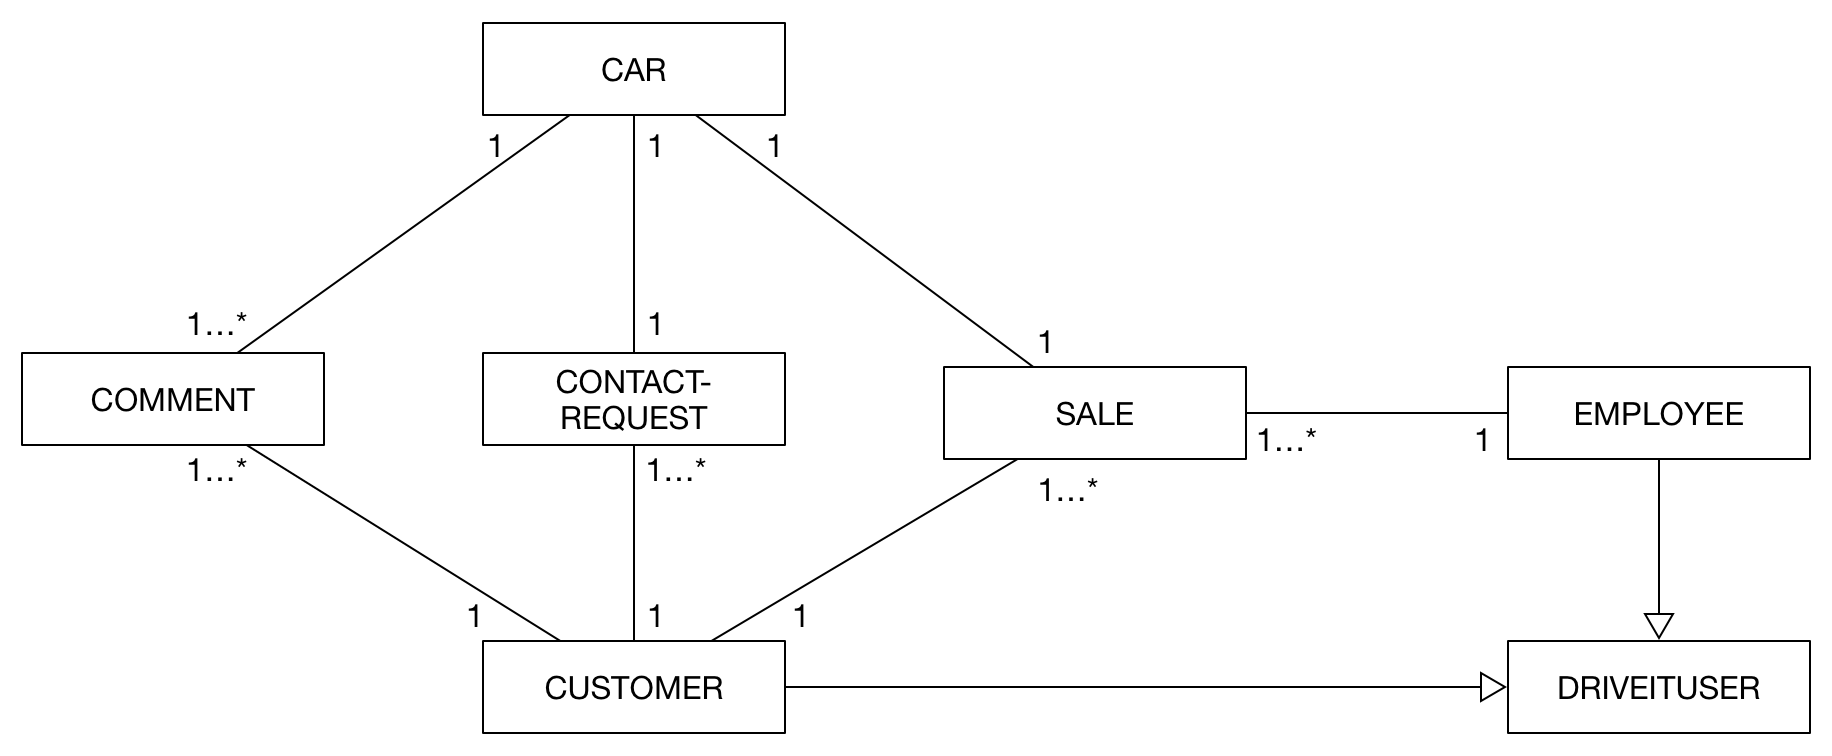
\includegraphics[width=\textwidth]{Figures/DomainObjectModel}\\
		% place the figure in the Figures folder (located with the main file)
		% you need to fix the scale a few times to get it right, but latex does not compress so one can always zoom in to see details.
	\caption{The Domain Object Model of the \texttt{DriveIT System}.}
  \label{fig:DomainObjectModel}
  % label it something meanfull
\end{figure}

The \texttt{Car} object is a given used car that the car lot has purchased. A \texttt{Car} can have many or no \texttt{Comment}s. A \texttt{Comment} has only one \texttt{Customer}, but one \texttt{Customer} can create many \texttt{Comment}s.

A \texttt{Customer} can create many \texttt{Contact Request}s, but a given \texttt{Contact Request} can only come from one \texttt{Customer}.

When a  \texttt{Car} is purchased a \texttt{Sale} is created. A \texttt{Sale} can only have one \texttt{Customer}, one \texttt{Car} and one \texttt{Employee}.

One \texttt{Customer} can have many sales (if he/she buys many cars), but a given \texttt{Car} can only be sold once. An \texttt{Employee} can likewise have sold many cars.\\ 
An \texttt{Employee} represents an employee working at the used car lot, selling \texttt{Car}s to \texttt{Customer}s. The employee is referenced in a \texttt{Sale} when selling a \texttt{Car}.  

The \texttt{Admin} inherits from the \texttt{Employee} but has some special rights in the system (see Access Control).